\section{Write the Constraints File}

    We now need to connect the LED pin to the GPIO\_0 port we just created. We will do this by writing a constraints file, which connects pins on the Zedboard to signals in our RTL design loaded onto the \gls{fpga}.

    \subsection{Constraints File Syntax}

    Vivado constraints files (\texttt{.xdc}) use Tcl syntax to assign physical and electrical properties to design objects such as ports. The general form is:

    \begin{verbatim}
    set_property <PROPERTY> <VALUE> [get_<object_type> <object_name>]
    \end{verbatim}

    For top-level I/O, the object type is \texttt{get\_ports}, where the port name must match the RTL design exactly. For example:

    \begin{verbatim}
    set_property PACKAGE_PIN T22 [get_ports {leds_o[0]}]
    set_property IOSTANDARD LVCMOS33 [get_ports {leds_o[0]}]
    \end{verbatim}

    Multiple properties can be assigned in a single command using \texttt{-dict}:

    \begin{verbatim}
    set_property -dict {PACKAGE_PIN T22 IOSTANDARD LVCMOS33} [get_ports {leds_o[0]}]
    \end{verbatim}

    Curly braces \{\} are used to group names (e.g. bus indices like \texttt{leds\_o[0]}) and prevent Tcl parsing issues.

    \paragraph{Key Points}
    \begin{itemize}
        \item Port names in \texttt{get\_ports} must exactly match the top-level design (case-sensitive).
        \item \texttt{PACKAGE\_PIN} and \texttt{IOSTANDARD} are device-specific properties defined by the FPGA and board.
        \item The order of constraints in the file is generally not important.
        \item Comments are written using \texttt{\#}.
    \end{itemize}

    To write our tcl:
    
    \begin{enumerate}
        \item Inside the project tree create a folder called constraints, and inside constraints a file entitled constraints.xdc. 
        \item We next need to refer to the Zedboard documentation at 
        \href{https://files.digilent.com/resources/programmable-logic/zedboard/ZedBoard_HW_UG_v2_2.pdf}{ZedBoard Hardware User Guide}, in order to understand which LED is connected to what Zynq pin, and the correct electrical characteristics. This information is found in section 2.7.3 on page 20.
        
        \begin{center}
            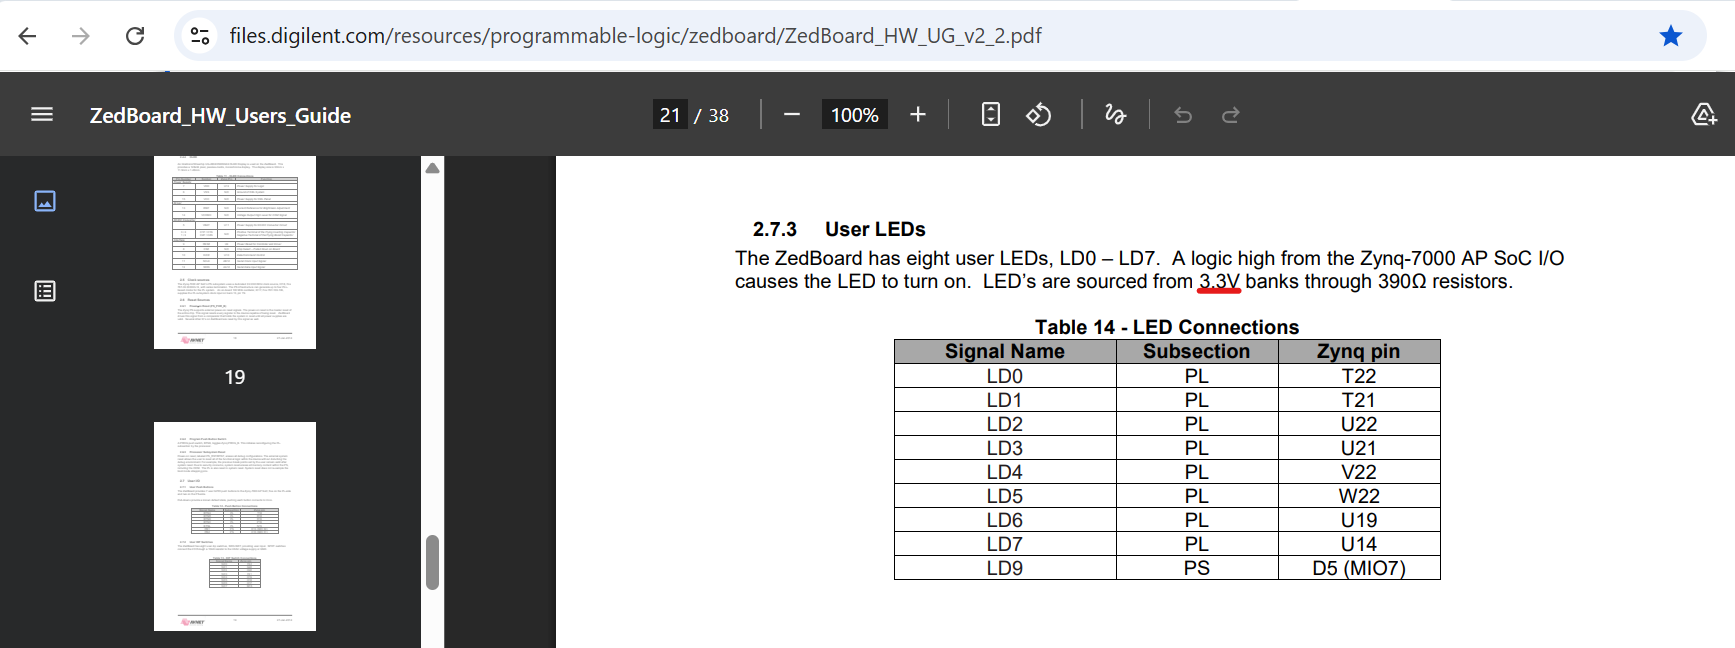
\includegraphics[width=0.9\textwidth]{aa_latex/Figures/Blink_LED/constraints/LEDs_zynq_pin.png}
        \end{center}

        \item We note that the LEDs are sourced from 3.3 V banks. This means each LED pin requiers the input output standard LCVMOSS 33. If we take Zynq pin T22 then, we have:
        
            \begin{verbatim}
                set_property PACKAGE_PIN T22 [get_ports {o_leds[0]}]
                set_property IOSTANDARD LVCMOS33 [get_ports {o_leds[0]}]
            \end{verbatim}
        
            \item the get\_ports name and index is decided by us. We could have used a different name, e.g.
            
                \begin{verbatim}
                    set_property PACKAGE_PIN T22 [get_ports {leds_out[0]}]
                    set_property IOSTANDARD LVCMOS33 [get_ports {leds_out[0]}]
                \end{verbatim}
            \item We can also using -dict to make it one line:
            
            \begin{verbatim}
                set_property -dict {PACKAGE_PIN T22 IOSTANDARD LVCMOS33} [get_ports {o_leds[0]}]
            \end{verbatim}

        \item Note, there is a zedboard\_master.xdc that can somewhat simplify the above process.        
    \end{enumerate} 